\documentclass[11pt]{beamer}
\usetheme{Malmoe}
\usefonttheme[onlymath]{serif}

\usepackage{graphicx} \usepackage{url} \usepackage{hyperref} \usepackage{caption} \usepackage{amsmath}
\usepackage{amssymb} \usepackage{array} \usepackage{listings} \usepackage{color} \usepackage{textcomp}
\usepackage[utf8]{inputenc} \usepackage{natbib} \usepackage{algorithm} \usepackage{tikz}
\usepackage[noend]{algpseudocode} \usepackage{csquotes}

\usetikzlibrary{shapes.geometric, arrows}

\setbeamercovered{transparent}
\setbeamertemplate{navigation symbols}{}
\setbeamerfont{page number in head/foot}{size=\fontsize{9}{11}}
\setbeamertemplate{footline}[frame number]
\setbeamertemplate{section in toc}{\inserttocsectionnumber.~\inserttocsection}

\author{Glenn Galvizo}
\title{Analysis of Lost-in-Space Star Identification Methods}
\institute{University of Hawaii at Manoa - Advisor: Dr. Lipyeow Lim}

\begin{document}
    \begin{frame}
        \titlepage
    \end{frame}

    \begin{frame}
        \frametitle{Overview}
        \tableofcontents
    \end{frame}

    \section{Background}\label{sec:background}
    \subsection{Problem Statement}\label{subsec:problemStatement}
    \begin{frame}
        \frametitle{Research Goal: Characterization}
        \begin{block}{Lost-in-Space Attitude Determination Process}
            \begin{enumerate}
                \item Given an image of stars \medskip
                \item Move stars to a 3D coordinate frame \medskip
                \item \textbf{Identify a select few stars in the image} \medskip
                \item Determine how we are oriented \medskip
            \end{enumerate}
        \end{block} \bigskip
        What is the most optimal identification process?
    \end{frame}

    \subsection{Importance}\label{subsec:importance}
    \begin{frame}
        \frametitle{Roots: Ancient Navigation}
        \centerline{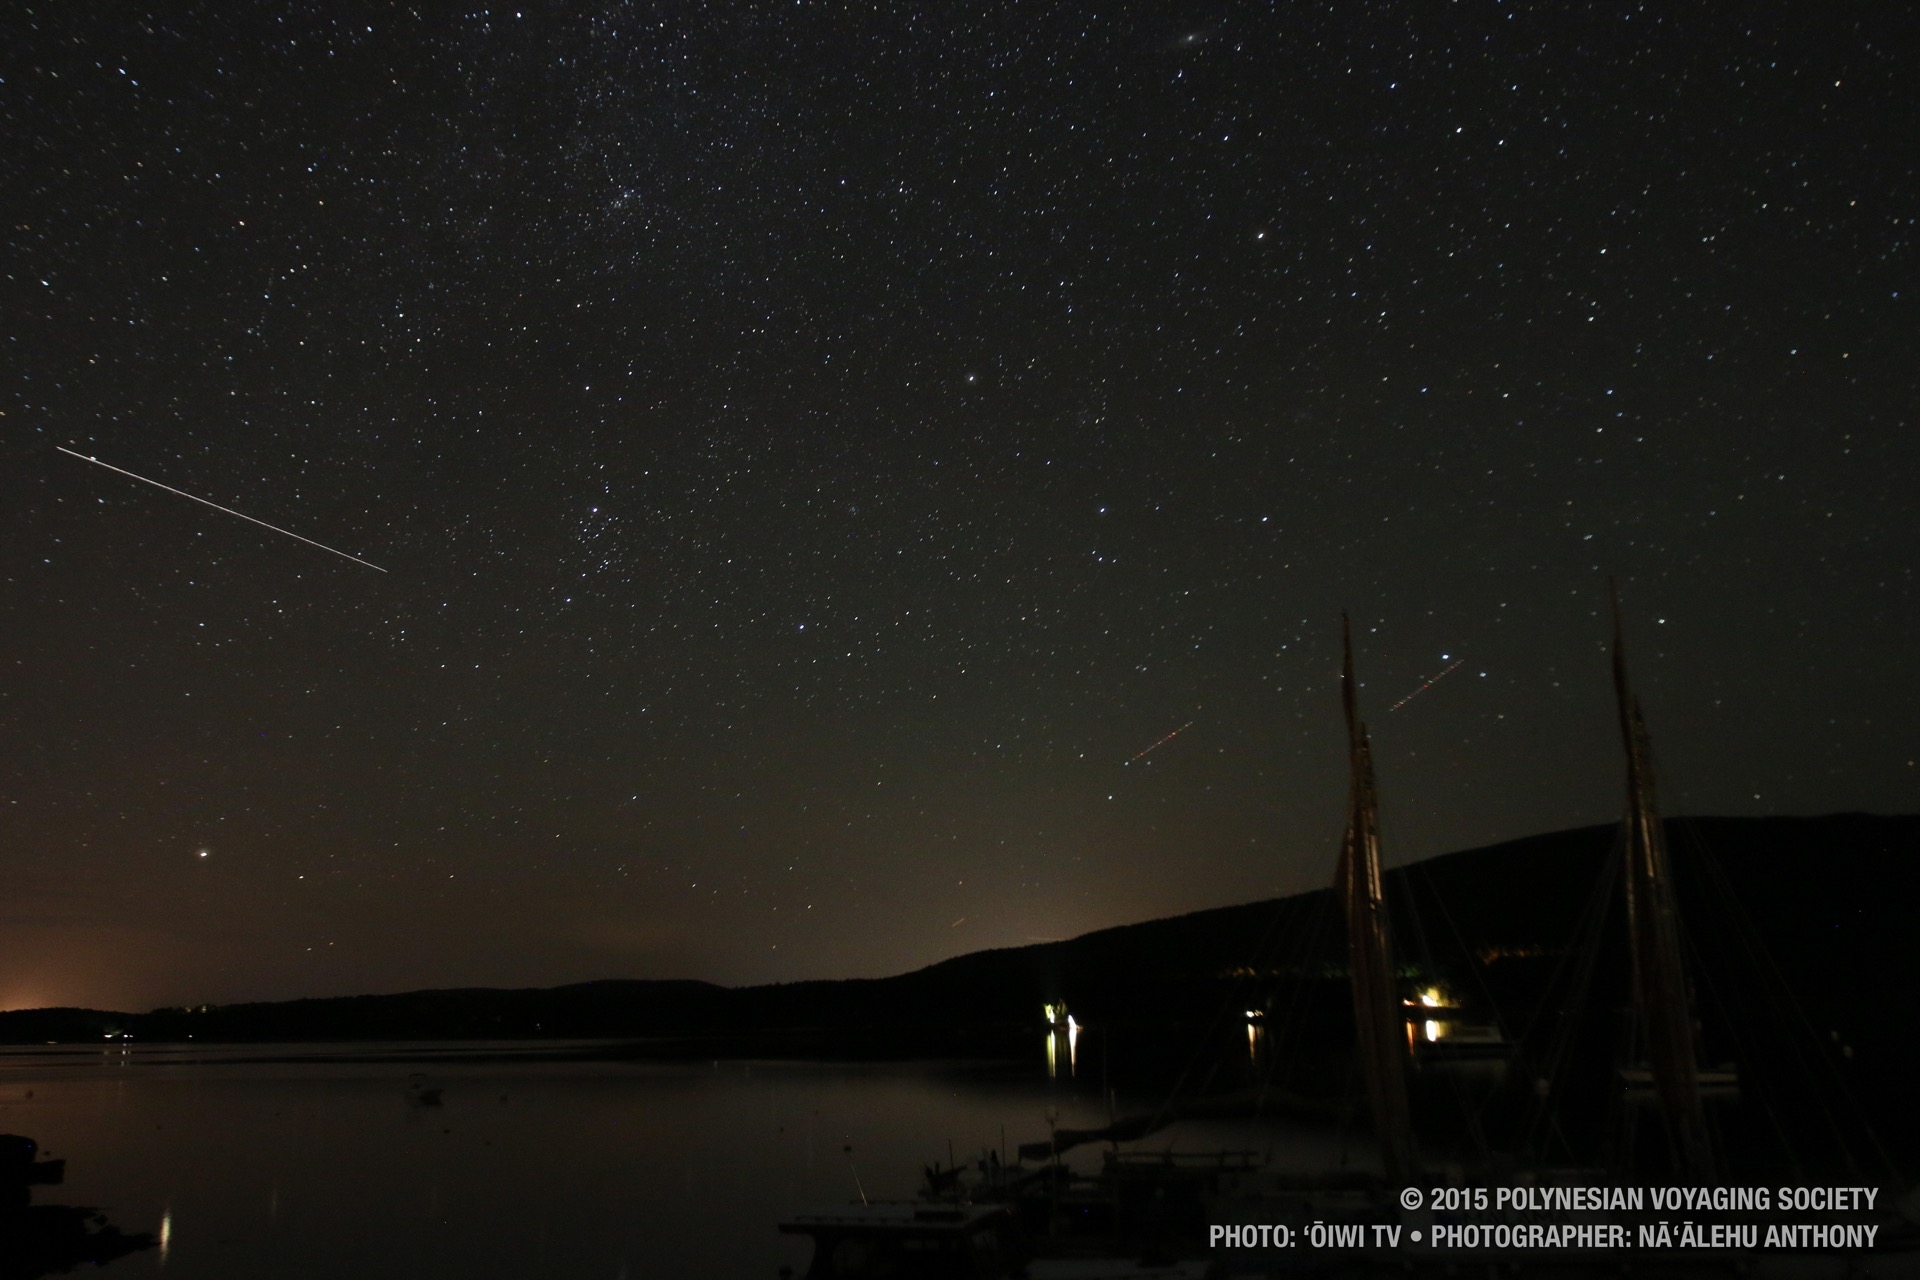
\includegraphics[scale=0.16]{images/hokulea}}
        \centerline{\textit{Stars provide a lot of positional information!}}
    \end{frame}

    % Taking a step back. Going to talk about attitude determination.
    \begin{frame}
        \frametitle{Relevancy: Spacecraft Attitude}
        \begin{definition}
            Attitude determination = process of finding one's \textit{orientation} in space
        \end{definition} \medskip
        \begin{columns}
            \begin{column}{0.5\textwidth}
                \begin{itemize}
                    \item Craft uses orientation to: \medskip
                    \begin{enumerate}
                        \item Orient solar panels
                        \item Direct thrusters
                        \item Position payload
                    \end{enumerate} \medskip
                    \item Ancient navigator analogy: \medskip
                    \begin{enumerate}
                        \item Navigator $\leftrightarrow$ Computer
                        \item Eyes $\leftrightarrow$ Camera
                        \item Methods $\leftrightarrow$ Algorithm
                    \end{enumerate}
                \end{itemize}
            \end{column}
            \begin{column}{0.5\textwidth}
                \centering{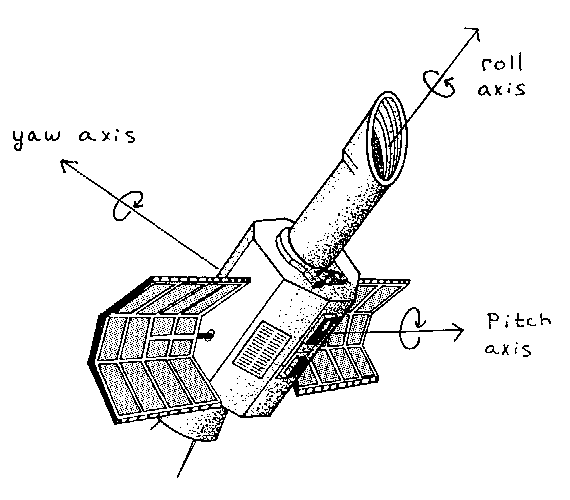
\includegraphics[scale=0.35]{images/spacecraft-attitude}}
            \end{column}
        \end{columns}
    \end{frame}

    \subsection{Spacecraft Attitude Problem}\label{subsec:spacecraftAttitudeProblem}
    \begin{frame}
        \frametitle{Attitude Determination}
        \begin{columns}
            \begin{column}{0.5\textwidth}
                \begin{itemize}
                    \item $A \gets$ inertial frame \bigskip
                    \item $B \gets$ body frame \bigskip
                    \item $X_A \gets$ known location in $A$ \bigskip
                    \item $X_B \gets$ observation in $B$ \bigskip
                \end{itemize}
            \end{column}
            \begin{column}{0.55\textwidth}
                \centering{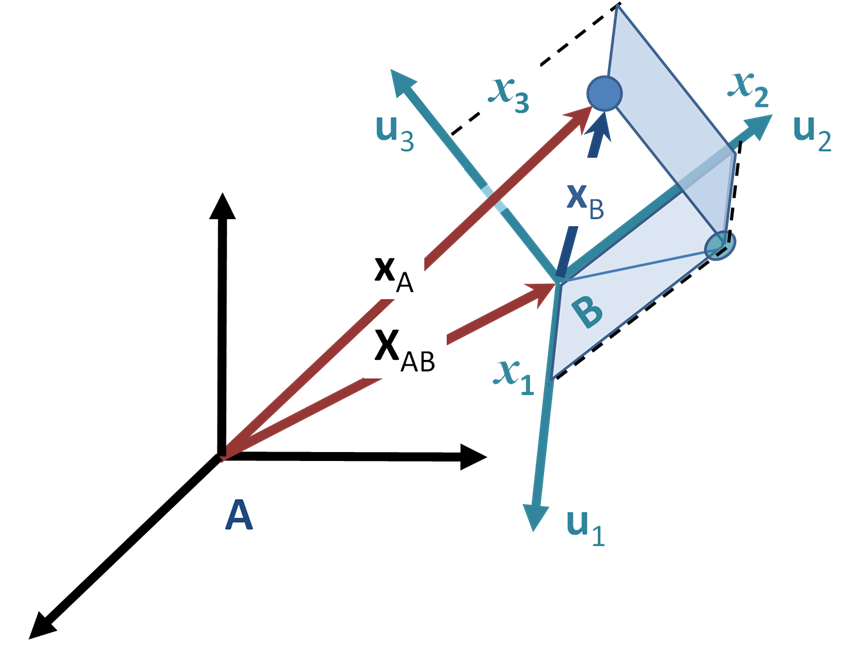
\includegraphics[scale=0.2]{images/moving-coordinate-systems.PNG}}
            \end{column}
        \end{columns} \bigskip
        \centering{\textit{Goal: Find rotation $X_{AB}$ to take $A$ points to $B$}}
    \end{frame}

    \begin{frame}
        \frametitle{Stellar Attitude Determination}
        \begin{columns}
            \begin{column}{0.5\textwidth}
                \centering{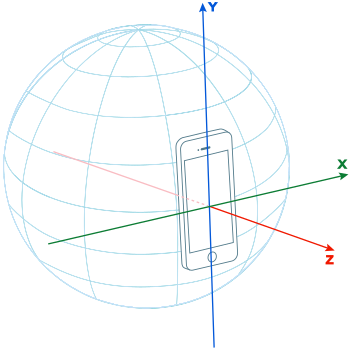
\includegraphics[scale=0.4]{images/phone-accelerometer.png}} \\
                \textbf{Earth: \\} Use Acceleration Toward Earth
            \end{column}
            \begin{column}{0.5\textwidth}
                \centering{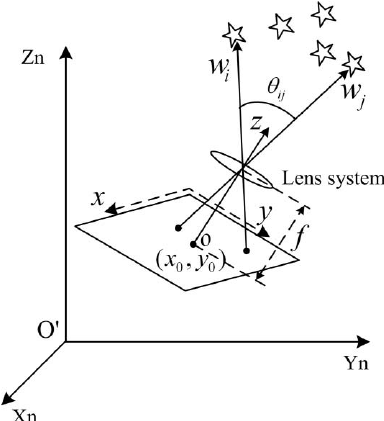
\includegraphics[scale=0.335]{images/star-tracker-lens.png}} \\
                \textbf{Space (LEO): \\} Use Stellar Objects (Sun, Stars)
            \end{column}
        \end{columns}
    \end{frame}

    \begin{frame}
        \frametitle{Wahba's Problem}
        \begin{definition}
            Wahba's Problem = Finding rotation $X_{AB}$ to take frame $A$ to $B$, using set of observations in both
            frames
        \end{definition} \bigskip
        \begin{itemize}
            \item Observations in $A$ are ($X_A, X'_A, X''_A, \ldots$) \medskip
            \item Observations in $B$ are ($X_B, X'_B, X''_B, \ldots$) \medskip
            \item $X_A$ maps to $X_B$, $X'_A$ maps to $X'_B$, \ldots \bigskip \bigskip
            \item \textbf{Requires two sets of observations to solve} \medskip
            \item Known approaches: TRIAD, Q-Method (Newton), QUEST
        \end{itemize}
    \end{frame}

    % https://www.w3.org/TR/orientation-sensor/images/absolute_orientation_sensor_coordinate_system.png
    % https://www.researchgate.net/profile/Haibo_Liu_12/publication/252685563/figure/fig1/AS:298171570900992
    %       @1448101050111/Fig-1-Measurement-model-of-star-tracker.png

    \section{Identification Algorithms}\label{sec:identificationAlgorithms}
    \begin{frame}
        \begin{block}{Question}
            How do we match image stars (body) to catalog stars (inertial)?
        \end{block}
        \begin{block}{Answer}
            A star identification algorithm!
        \end{block}
        \begin{figure}
            \hspace*{-30pt}\centering{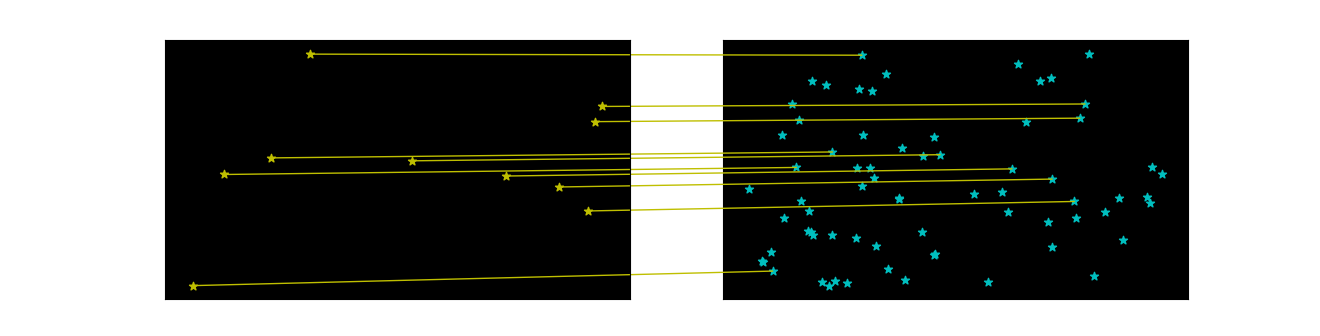
\includegraphics[scale=0.37]{images/star-identification.png}}
            \caption{Depicts mapping of stars in image (left, in yellow) to stars in catalog (right, in blue)}
        \end{figure}
    \end{frame}

    \subsection{Generic Identification}\label{subsec:genericIdentification}
    \begin{frame}
        \begin{figure}
            \begin{columns}
                \begin{column}{0.4\linewidth}
                    \centering{\scalebox{.53}{% Style for process block.
\tikzstyle{process} = [rectangle, text width=3cm, minimum width=3cm, minimum height=1cm,text centered, draw=black,
fill=orange!30]

% Style for terminal block.
\tikzstyle{terminal} = [rectangle, text width=1.7cm, minimum width=1.7cm, minimum height=1.7cm,text centered,
draw=black, fill=red!30]

% Style for decision block.
\tikzstyle{decision} = [diamond, text width=2cm, minimum width=2.5cm, minimum height=2.5cm,text centered, draw=black,
fill=green!30, inner sep=-10pt]

% Style for line.
\tikzstyle{line} = [draw, -latex']

\begin{tikzpicture}[node distance=1.8cm]
    \node[scale=1](getImage)[terminal]{Get Camera Image};
    \node[scale=1](pickQueryStars) [process, left of=getImage, xshift = -1.7cm] {Pick $k$ Image Stars};
    \node[scale=1](searchCatalog)[process, below of=pickQueryStars] {Search Catalog};
    \node[scale=1](confidentInCatalog)[decision, below of=searchCatalog, yshift=-0.5cm] {$|R| > 0$?};
    \node[scale=1](filterCandidates)[process, below of=confidentInCatalog, yshift=-0.5cm] {Filter Candidates};
    \node[scale=1](confidentAfterFilter)[decision, below of=filterCandidates, yshift=-0.5cm] {Confident in $r$?};
    \node[scale=1](findMap)[process, below of=confidentAfterFilter, yshift=-0.5cm]{Identify};
    \node[scale=1](confidentInMap)[decision, below of=findMap, yshift=-0.5cm] {Confident in $a$?};
    \node[scale=1](returnMap)[terminal, right of=confidentInMap, xshift = 1.7cm] {Return Map};

    \draw[->,>=stealth](getImage) -- node[scale=1.3, yshift=-0.3cm]{$I$}(pickQueryStars);
    \draw[->,>=stealth] (pickQueryStars) -- node[scale=1.3, xshift=0.5cm]{$b$}(searchCatalog);
    \draw[->, >=stealth] (searchCatalog) -- node[scale=1.3, xshift=0.5cm, yshift=-0.15cm]{$R$}(confidentInCatalog);
    \draw[->, >=stealth] (confidentInCatalog) -- node[anchor=east, yshift=0.1cm]{Yes}(filterCandidates);
    \draw[->, >=stealth] (filterCandidates) -- node[scale=1.3, xshift=0.5cm, yshift=-0.15cm]{$r$}(confidentAfterFilter);
    \draw[->, >=stealth] (confidentInMap) -- node[xshift=-0.05cm, yshift=0.2cm]{Yes}(returnMap);
    \draw[->, >=stealth] (confidentAfterFilter) -- node[anchor=east, yshift=0.1cm]{Yes} (findMap);
    \draw[->, >=stealth] (findMap) -- node[scale=1.3, xshift=0.5cm, yshift=-0.15cm]{$a$}(confidentInMap);

    \draw[->, >=stealth] (confidentInCatalog.west) -- ++(-1.1cm, 0cm) node[anchor=south, xshift=0.5cm]{No}
    |- (pickQueryStars.west);
    \draw[->, >=stealth] (confidentAfterFilter.west) -- ++(-1.1cm, 0cm) node[anchor=south, xshift=0.5cm]{No}
    |- (pickQueryStars.west);
    \draw[->, >=stealth](confidentInMap.west) -- ++(-1.1cm, 0cm) node[anchor=south, xshift=0.5cm]{No}
    |- (pickQueryStars.west);
\end{tikzpicture}}}
                \end{column}
                \begin{column}{0.6\linewidth}
                    \caption{Flowchart depicting flow of general identification method} \bigskip
                    \begin{enumerate}
                        \item \textit{Search Catalog} $=$ Query w/ Features Step \medskip
                        \item \textit{Filter Candidates} $=$ Reduction Step \medskip
                        \item \textit{Identify} $=$ Identification Step \medskip
                        \item \textit{\textbf{Requires $|I| \geq 3$}} \medskip
                    \end{enumerate}
                \end{column}
            \end{columns}
        \end{figure}
    \end{frame}

    \subsection{Existing Implementations}\label{subsec:existingImplementations}
    \begin{frame}
        \frametitle{Popular Approaches to Star Identification}
        \begin{table}
            \centering{\tiny\hspace*{-10pt}\begin{tabular}{  m{0.22\linewidth} || m{0.21\linewidth} | m{0.21\linewidth} | m{0.24\linewidth} }
    & \textbf{Image Features} & \textbf{Reduction} & \textbf{Identification} \\
    \hline \hline
    \textbf{Angle} & $\theta^{ij}$ & Require $\lvert R \rvert=1$ & \Call{DMT}{$b, r, I$} \\ \hline
    \textbf{Dot Angle} & $\theta^{ic}, \theta^{jc}, \phi$ & Require $\lvert R \rvert = 1$ & Restrict $\theta^{ic},
    \theta^{jc}$ at Query Time \\ \hline
    \textbf{Spherical Triangle} & Spherical $a^{ijk}, \imath^{ijk}$ & \Call{Pivot}{$b_i, b_j, b_k, R_1$} &
    \Call{DMT}{$b, r, I$} \\ \hline
    \textbf{Planar Triangle} & Planar $a^{ijk}, \imath^{ijk}$ & \Call{Pivot}{$b_i, b_j, b_k, R_1$} &
    \Call{DMT}{$b, r, I$} \\ \hline
    \textbf{Pyramid} & $\theta^{ij}, \theta^{ik}, \theta^{jk}$ & Require $\lvert R \rvert = 1$ &
    \Call{Common}{$R^{ab}, R^{ac}, F$}, \newline \Call{PyramidVerify}{$r, b, I$} \\ \hline
    \textbf{Composite Pyramid} & Planar $a^{ijk}, \imath^{ijk}$ & Require $\lvert R \rvert = 1$ & \Call{DMT}{$b, r, I$},
    \newline \Call{CompositeVerify}{$r, b, a, I$}
\end{tabular}
} \bigskip \bigskip
            \centering{
            \caption{
            Overview table of the different identification methods.
            Each method's image features, reduction process, identification process is displayed.
            } \label{tab:identificationMethodOverview}
            }
        \end{table}
    \end{frame}

    \section{Methodology}\label{sec:methodology}
    \begin{frame}
        \frametitle{Experiment Overview}
        \begin{block}{Research Goal}
            What is the most optimal identification process?
        \end{block} \bigskip \bigskip
        Which method has the best \ldots.
        \begin{enumerate}
            \item Query process? \medskip
            \item Reduction process? \medskip
            \item Identification process? \medskip
        \end{enumerate}
    \end{frame}

    \subsection{Image Generation}\label{subsec:imageGeneration}
    \begin{frame}
        \frametitle{Benchmark Image Generation}
        \begin{columns}
            \begin{column}{0.5\textwidth}
                \begin{block}{Problem}
                    Gathering image data and characterizing error is hard :(
                \end{block} \medskip
                \begin{block}{Solution}
                    Generate artifical images!
                    \begin{itemize}
                        \item Uses real stars from Hipparcos star catalogue
                        \item Work entirely in 3D frame
                        \item An image center and field-of-view are specified
                        \item Can apply artificial error (centroiding, false stars)
                    \end{itemize}
                \end{block}
            \end{column}
            \begin{column}{0.5\textwidth}
                \hspace*{-2pt}\centering{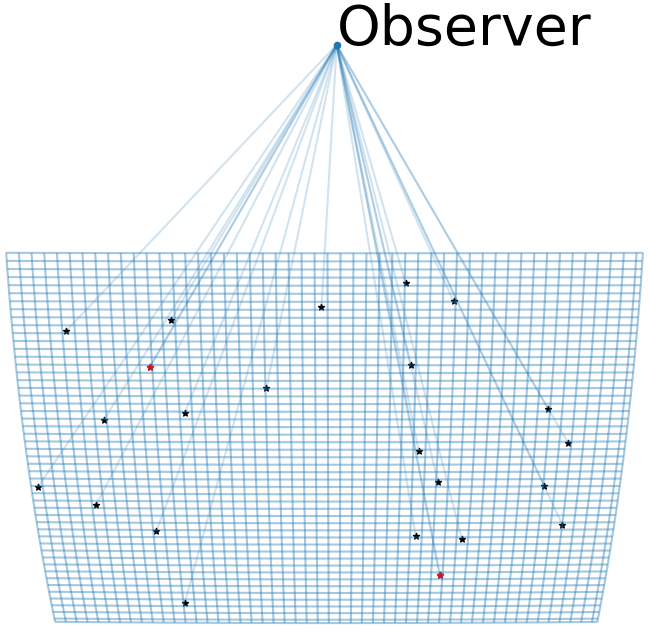
\includegraphics[scale=0.3]{images/benchmark.png}}
            \end{column}
        \end{columns}
    \end{frame}

    \subsection{Query Experiment}\label{subsec:queryExperiment}
    \begin{frame}
        \frametitle{Query Experiment}
        \begin{block}{Question}
            Which set of features most accurately distinguish a set of stars?
        \end{block}
        \begin{block}{Experiment}
            \begin{enumerate}
                \item Generate image of stars $I$
                \item Apply noise to image
                \item Run identification before reduction step (giving $R$) \underline{once}
                \item Check if $R$ contains the correct stars (denoted \textit{hit})
                \item Repeat for different image
            \end{enumerate}
        \end{block}
        \begin{block}{Analysis}
            More hits and smaller $\lvert R \rvert$ $\rightarrow$ effective filter
        \end{block}
    \end{frame}

    \begin{frame}
        \begin{figure}
            \begin{columns}
                \begin{column}{0.4\linewidth}
                    \centering{\scalebox{.53}{% Style for process block.
\tikzstyle{process} = [rectangle, text width=3cm, minimum width=3cm, minimum height=1cm,text centered, draw=black,
fill=orange!30]

% Style for terminal block.
\tikzstyle{terminal} = [rectangle, text width=1.7cm, minimum width=1.7cm, minimum height=1.7cm,text centered,
draw=black, fill=red!30]

% Style for decision block.
\tikzstyle{decision} = [diamond, text width=2cm, minimum width=2.5cm, minimum height=2.5cm,text centered, draw=black,
fill=green!30, inner sep=-10pt]

% Style for line.
\tikzstyle{line} = [draw, -latex']

\begin{tikzpicture}[node distance=1.8cm]
    \node[scale=1](getImage)[terminal]{Get Camera Image};
    \node[scale=1](pickQueryStars) [process, left of=getImage, xshift = -1.7cm] {Pick $k$ Image Stars};
    \node[scale=1](searchCatalog)[process, below of=pickQueryStars] {Search Catalog};
    \node[scale=1](confidentInCatalog)[decision, below of=searchCatalog, yshift=-0.5cm] {$|R| > 0$?};
    \node[scale=1](filterCandidates)[process, below of=confidentInCatalog, yshift=-0.5cm] {Filter Candidates};
    \node[scale=1](confidentAfterFilter)[decision, below of=filterCandidates, yshift=-0.5cm] {Confident in $r$?};
    \node[scale=1](findMap)[process, below of=confidentAfterFilter, yshift=-0.5cm]{Identify};
    \node[scale=1](confidentInMap)[decision, below of=findMap, yshift=-0.5cm] {Confident in $a$?};
    \node[scale=1](returnMap)[terminal, right of=confidentInMap, xshift = 1.7cm] {Return Map};

    \draw[->,>=stealth](getImage) -- node[scale=1.3, yshift=-0.3cm]{$I$}(pickQueryStars);
    \draw[->,>=stealth] (pickQueryStars) -- node[scale=1.3, xshift=0.5cm]{$b$}(searchCatalog);
    \draw[->, >=stealth] (searchCatalog) -- node[scale=1.3, xshift=0.5cm, yshift=-0.15cm]{$R$}(confidentInCatalog);
    \draw[->, >=stealth] (confidentInCatalog) -- node[anchor=east, yshift=0.1cm]{Yes}(filterCandidates);
    \draw[->, >=stealth] (filterCandidates) -- node[scale=1.3, xshift=0.5cm, yshift=-0.15cm]{$r$}(confidentAfterFilter);
    \draw[->, >=stealth] (confidentInMap) -- node[xshift=-0.05cm, yshift=0.2cm]{Yes}(returnMap);
    \draw[->, >=stealth] (confidentAfterFilter) -- node[anchor=east, yshift=0.1cm]{Yes} (findMap);
    \draw[->, >=stealth] (findMap) -- node[scale=1.3, xshift=0.5cm, yshift=-0.15cm]{$a$}(confidentInMap);

    \draw[->, >=stealth] (confidentInCatalog.west) -- ++(-1.1cm, 0cm) node[anchor=south, xshift=0.5cm]{No}
    |- (pickQueryStars.west);
    \draw[->, >=stealth] (confidentAfterFilter.west) -- ++(-1.1cm, 0cm) node[anchor=south, xshift=0.5cm]{No}
    |- (pickQueryStars.west);
    \draw[->, >=stealth](confidentInMap.west) -- ++(-1.1cm, 0cm) node[anchor=south, xshift=0.5cm]{No}
    |- (pickQueryStars.west);
\end{tikzpicture}}}
                \end{column}
                \begin{column}{0.6\linewidth}
                    \caption{Flowchart depicting flow of general identification method} \bigskip
                    \begin{enumerate}
                        \item \textit{Search Catalog} $=$ Query w/ Features Step \medskip
                        \item \textit{Filter Candidates} $=$ Reduction Step \medskip
                        \item \textit{Identify} $=$ Identification Step \medskip
                    \end{enumerate}
                \end{column}
            \end{columns}
        \end{figure}
    \end{frame}

    \subsection{Reduction Experiment}\label{subsec:reductionExperiment}
    \begin{frame}
        \frametitle{Reduction Experiment}
        \begin{block}{Question}
            What is the best process for reducing a set of catalog candidates?
        \end{block}
        \begin{block}{Experiment}
            \begin{enumerate}
                \item Generate image of stars $I$
                \item Apply noise to image
                \item Run identification before identification step (giving $r$)
                \item Check if $r$ contains correct stars in $I$ (\textit{hits})
                \item Repeat for different image
            \end{enumerate}
        \end{block}
        \begin{block}{Analysis}
            Characterize reduction process, more hits $\rightarrow$ less false negatives
        \end{block}
    \end{frame}

    \subsection{Identification Experiment}\label{subsec:identificationExperiment}
    \begin{frame}
        \frametitle{Identification Experiment}
        \begin{block}{Question}
            Which identification method can most accurately determine a map?
        \end{block}
        \begin{block}{Experiment}
            \begin{enumerate}
                \item Generate image of stars $I$
                \item Apply noise to image
                \item Run identification method end to end (giving $a$)
                \item Check if $a$ is a correct map (\textit{hits})
                \item Repeat for different image
            \end{enumerate}
        \end{block}
        \begin{block}{Analysis}
            Characterize mapping process, more hits $\rightarrow$ accurate mapping
        \end{block}
    \end{frame}

    \section{Conclusion}\label{sec:conclusion}
    \begin{frame}
        \frametitle{Conclusion}
        \begin{block}{Research Goal}
            Determine what is the most optimal identification method
        \end{block} \medskip
        \begin{block}{Spacecraft Attitude Problem}
            Given ($X_A, X'_A, \ldots$) and ($X_B, X'B, \ldots$), find $X_{AB}$
        \end{block} \medskip
        \begin{block}{Star Identification}
            Determine mapping $X_A \rightarrow X_B$, $X'_A \rightarrow X'_B, \ldots$
        \end{block} \medskip
        \begin{block}{Methodology}
            Characterize \textit{query}, \textit{reduction}, and \textit{identification}
        \end{block}
    \end{frame}

    \begin{frame}
        \frametitle{Acknowledgments}
        \begin{itemize}
            \item Dr. Lipyeow Lim \medskip
            \item Hawaii Space Flight Laboratory \medskip
            \item Undergraduate Research Opportunities Program \medskip
            \item Undergraduate Showcase \medskip
            \item The Audience \medskip
        \end{itemize}
    \end{frame}

    \begin{frame}
        \centering{\huge{Questions?}}
    \end{frame}
\end{document}
